\section*{Đề kiểm tra Chương 8}
\subsection*{Đề số 1}
\setcounter{ex}{0}\setcounter{bt}{0}
\Opensolutionfile{ans}[ans/ans-KT-801]
\noindent\textbf{I. PHẦN TRẮC NGHIỆM}
\begin{ex}%[Hữu Bình - BG Toán 10]%[1D2Y1-1]
	Trên giá sách có $ 8 $ quyển sách Văn và $ 10 $ quyển sách Toán, các quyển này đôi một khác nhau. Hỏi có bao nhiêu cách chọn ra $ 1 $ quyển sách trên giá?
	\choice
	{$ 80 $}
	{$ 10 $}
	{$ 8 $}
	{\True $ 18 $}
	\loigiai{
		Số cách chọn 1 quyển sách Văn là $ 8 $.\\
		Số cách chọn $ 1 $ quyển sách Toán là $ 10 $.\\
		Số cách chọn 1 quyển sách là $ 8+10=18 $ cách.
	}
\end{ex}
\begin{ex}%[Hữu Bình - BG Toán 10]%[1D2Y1-1]
	Từ một bó hoa hồng gồm $3$ bông hồng trắng, $5$ bông hồng đỏ và $6$ bông hồng vàng, có bao nhiêu cách chọn ra một bông hồng?
	\choice
	{$90$}
	{$8$}
	{$11$}
	{\True $14$}
	\loigiai{
		Chọn $1$ bông hồng trắng có: $3$ cách chọn.\\
		Chọn $1$ bông hồng đỏ có: $5$ cách chọn.\\
		Chọn $1$ bông hồng vàng có: $6$ cách chọn.\\
		Do đó, theo quy tắc cộng có $3+5+6=14$ cách chọn $1$ bông hồng.
	}
\end{ex}

\begin{ex}%[Hữu Bình - BG Toán 10]%[1D2Y1-1]
	Một hộp có $ 9 $ bóng đèn màu xanh, $ 7 $ bóng đèn màu đỏ. Số cách chọn một bóng đèn bất kỳ trong hộp đó là 
	\choice
	{$ 36 $}
	{$ 61 $}
	{$ 63 $}
	{\True $ 16 $}
	\loigiai{
		Số cách chọn một bóng đèn bất kỳ trong hộp là $ 9+7=16 $.
	}
\end{ex}
\begin{ex}%[Hữu Bình - BG Toán 10]%[1D2Y1-2]
	Một lớp học có $19$ bạn nữ và $16$ bạn nam. Hỏi có bao nhiêu cách chọn ra $2$ bạn, trong đó có $1$ bạn nam và $1$ bạn nữ?
	\choice
	{$35$ cách}
	{$595$ cách}
	{\True $304$ cách}
	{$1190$ cách}
	\loigiai{ Có $19$ cách chọn $1$ bạn nữ từ $19$ bạn nữ và $16$ cách chọn $1$ bạn nam từ $16$ bạn nam.\\
		Vậy số cách chọn là $19\cdot 16=304$ cách.
	}
\end{ex}
\begin{ex}%[Hữu Bình - BG Toán 10]%[1D2Y1-1]
	\immini{Các tỉnh $A$, $B$, $C$ được nối với nhau bởi các con đường như hình vẽ. Hỏi có tất cả bao nhiêu cách để đi từ tỉnh $A$ đến tỉnh $C$ mà chỉ qua tỉnh $B$ chỉ một lần?
		\choice
		{$5$}
		{\True $6$}
		{$7$}
		{$8$}}{
		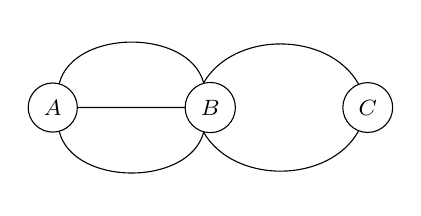
\begin{tikzpicture}[scale=1, font=\footnotesize, line join=round, line cap=round, >=stealth]
			\node[circle,draw] 	(A) at (0,0){$A$};
			\node[circle,draw] (B) at (2,0){$B$};
			\node[circle,draw] (C) at (4,0){$C$};
			\draw
			(A)--(B)
			(A)to[bend left=75](B)to[bend left=60](C)
			(A)to[bend right=75](B)to[bend right=60](C)
			;
		\end{tikzpicture}
	}
	\loigiai{
		Để đi từ tỉnh $A$ đến tỉnh $B$ có $3$ cách.\\
		Để đi từ tỉnh $B$ đến tỉnh $C$ có $2$ cách.\\
		Theo quy tắc nhân: Để đi từ tỉnh $A$ đến $C$ có: $3\times 2=6$ (cách).}
\end{ex}

\begin{ex}%[Hữu Bình - BG Toán 10]%[1D2Y1-2]  
	Từ tập $A=\left\{{1;2;3;4;5}\right\}$ có thể lập được bao nhiêu số tự nhiên lẻ có hai chữ số khác nhau?
	\choice
	{$15$}
	{$60$}
	{$20$}
	{\True $12$}
	\loigiai{
		Chữ số hàng đơn vị có $3$ cách chọn. Chữ số chục có $4$ cách chọn.\\
		Vậy có tất cả $3\cdot 4=12$ số tự nhiên lẻ có hai chữ số khác nhau.
	}
\end{ex}

\begin{ex}%[Hữu Bình - BG Toán 10]%[1D2Y1-2]
	Một tổ có $12$	học sinh. Đầu năm cô giáo chủ nhiệm cần chọn $1$ bạn làm tổ trưởng và $1$ bạn làm tổ phó. Hỏi có bao nhiêu cách chọn?
	\choice
	{$12!$}
	{\True $132$}
	{$66$}
	{$6$}
	\loigiai{
		Số cách chọn ra một học sinh làm tổ trưởng và một học sinh làm tổ phó là: $12 \cdot 11 = 132$ cách.
	}	
\end{ex}



\begin{ex}%[Hữu Bình - BG Toán 10]%[1D2B1-2]
	Một lớp học gồm có $20$ học sinh nam và $15$ học sinh nữ. Cần chọn ra $2$ học sinh gồm $1$ nam và $1$ nữ để phân công trực nhật. Số cách chọn là
	\choice
	{\True $300$}
	{$\mathrm{C}_{35}^2$}
	{$300$}
	{$\mathrm{A}_{35}^2$}
	\loigiai{
		Có $20$ cách chọn $1$ học sinh nam và $15$ cách chọn $1$ học sinh nữ. Do đó, ta có: $20\cdot 15=300$ cách chọn thỏa mãn yêu cầu bài toán.
	}
\end{ex}

\begin{ex}%[Hữu Bình - BG Toán 10]%[1D2B1-3]
	Từ một tập hợp gồm $ 10 $ câu hỏi, trong đó có $ 4 $ câu lý thuyết và $ 6 $ câu bài tập, người ta tạo thành các đề thi. Biết rằng một đề thi phải gồm $ 3 $ câu hỏi trong đó có ít nhất $ 1 $ câu lý thuyết và $ 1 $ câu bài tập. Hỏi có thể tạo được bao nhiêu đề khác nhau?
	\choice
	{$ 100 $}
	{$ 36 $}
	{\True $ 96 $}
	{$ 60 $}
	\loigiai{
		\begin{enumerate}
			\item[TH1.] Đề thi gồm $ 1 $ câu lý thuyết và $ 2 $ câu bài tập $ \Rightarrow $ số cách tạo ra đề thi là $ \mathrm{C}_{4}^{1}\cdot \mathrm{C}_{6}^{2} $ cách.
			\item[TH2.] Đề thi gồm $ 2 $ câu lý thuyết và $ 1 $ câu bài tập $ \Rightarrow $ số cách tạo ra đề thi là $ \mathrm{C}_{4}^{2}\cdot \mathrm{C}_{6}^{1} $ cách.
		\end{enumerate}
		Số đề được tạo ra là $ \mathrm{C}_{4}^{1}\cdot \mathrm{C}_{6}^{2}+\mathrm{C}_{4}^{2}\cdot \mathrm{C}_{6}^{1}=96 $ đề.
	}
\end{ex}
\begin{ex}%[Hữu Bình - BG Toán 10]%[1D2B1-3]
	Câu lạc bộ Tiếng Anh của trường THPT Triệu Sơn $2$ có $68$ thành viên, trong đó có $23$ nam và $45$ nữ. Trong buổi sinh hoạt hàng tháng cần chọn ra $2$ thành viên gồm $1$ nam và một nữ để dẫn chương trình, trong đó $1$ bạn dẫn bằng Tiếng Anh và $1$ bạn dẫn bằng Tiếng Việt. Hỏi có bao nhiêu sự lựa chọn?
	\choice
	{$1035$}
	{\True $2070$}
	{$2278$}
	{$4556$}
	\loigiai{
		\begin{itemize}
			\item Chọn bạn nam dẫn bằng Tiếng Anh, bạn nữ dẫn bằng Tiếng Việt có  $23\cdot 45 =1035$ (cách).
			\item Chọn bạn nữ dẫn bằng Tiếng Anh, bạn nam dẫn bằng Tiếng Việt có  $45\cdot 23 =1035$ (cách).
		\end{itemize}
		Số cách chọn thỏa mãn là $2070$ (cách).
	}
\end{ex}
\begin{ex}%[Hữu Bình - BG Toán 10]%[1D2B1-3]
	Cho hai đường thẳng song song $a$ và $b$. Trên đường thẳng $a$ có $5$ điểm phân biệt, trên đường thẳng $b$ có $7$ điểm phân biệt. Tính số tam giác có $3$ đỉnh lấy từ các điểm trên hai đường thẳng $a$ và $b$.
	\choice
	{\True $175$ tam giác}
	{$220$ tam giác}
	{$45$ tam giác}
	{$350$ tam giác}
	\loigiai{
		$\bullet$ Tam giác có $1$ đỉnh thuộc đường thẳng $a$ và $2$ đỉnh thuộc $b$, có $5\cdot \mathrm{C}_7^2=105$ tam giác.\\
		$\bullet$ Tam giác có $2$ đỉnh thuộc đường thẳng $a$ và $1$ đỉnh thuộc $b$, có $\mathrm{C}_5^2\cdot 7=70$ tam giác.\\
		Vậy tất cả có $105+70=175$ tam giác.
	}
\end{ex}
\begin{ex}%[Hữu Bình - BG Toán 10]%[1D2B1-3]
	Có hai chiếc hộp chứa bi. Hộp thứ nhất chứa $4$ viên bi đỏ và $3$ viên bi trắng, hộp thứ hai chứa $2$ viên bi đỏ và $4$ viên bi trắng. Lấy ngẫu nhiên từ mỗi hộp ra một viên. Có bao nhiêu cách lấy được $2$ viên bi cùng màu?
	\choice
	{\True $20$}
	{$16$}
	{$36$}
	{$22$}
	\loigiai{TH $1$: Lấy được $2$ viên bi đỏ có $4 \cdot 2=8$ cách.\\
		TH $2$: Lấy được $2$ viên bi trắng có $3 \cdot 4 =12$ cách.\\
		Theo qui tắc cộng ta có $8+12=20$ cách.}
\end{ex}
\begin{ex}%[Hữu Bình - BG Toán 10]%[1D2B1-3]
	Một bó hoa có $14$ bông hoa gồm: $3$ bông màu hồng, $5$ bông màu xanh còn lại là màu vàng. Hỏi có bao nhiêu cách chọn $7$ bông trong đó phải có đủ ba màu?
	\choice
	{\True $3058$}
	{$3060$}
	{$3432$}
	{$129$}
	\loigiai{
		Chọn $7$ bông bất kì từ $14$ bông có: $\mathrm{C}_{14}^7=3432$ cách.\\
		Chọn hai màu hồng, xanh có $\mathrm{C}_3^3 \cdot \mathrm{C}_5^4+\mathrm{C}_3^2 \cdot \mathrm{C}_5^5=8$ cách.\\
		Chọn hai màu hồng, vàng có $\mathrm{C}_3^3 \cdot \mathrm{C}_6^4+\mathrm{C}_3^2 \cdot \mathrm{C}_6^5+\mathrm{C}_3^1 \cdot \mathrm{C}_6^6=36$ cách.\\
		Chọn hai màu xanh, vàng có $\mathrm{C}_5^5 \cdot \mathrm{C}_6^2+\mathrm{C}_5^4 \cdot \mathrm{C}_6^3+\mathrm{C}_5^3 \cdot \mathrm{C}_6^4+\mathrm{C}_5^2 \cdot \mathrm{C}_6^5+\mathrm{C}_5^1 \cdot \mathrm{C}_6^6=330$ cách.\\
		Vậy có $3432-(8+36+330)=3058$ cách.}
\end{ex}

\begin{ex}%[Hữu Bình - BG Toán 10]%[1D2Y2-1]
	Giả sử có bảy bông hoa khác nhau và ba lọ hoa khác nhau. Hỏi có bao nhiêu cách cắm ba bông hoa vào ba lọ đã cho (mỗi lọ cắm một bông)?
	\choice
	{$35$}
	{$30240$}
	{\True $210$}
	{$21$}
	\loigiai{
		Số cách xếp bảy bông hoa khác nhau vào ba lọ hoa khác nhau là một chỉnh hợp chập $3$ của $ 7 $ phần tử. Suy ra có $ \mathrm{A}_7^3=210$ cách.}
\end{ex}

\begin{ex}%[Hữu Bình - BG Toán 10]%[1D2Y2-1]
	Một lớp học có $40$ học sinh. Chọn $3$ học sinh để tham gia vệ sinh công cộng toàn trường, hỏi có bao nhiêu cách chọn như trên?
	\choice
	{\True $ 9880$}
	{$ 59280$}
	{$ 2300$}
	{$ 455$}
	\loigiai{
		\\
		Nhóm học sinh $3$ người được chọn là một tổ hợp chập  $3$ của $40$ (học sinh).\\
		Vì vậy, số cách chọn nhóm học sinh là $ \mathrm{C}_{40}^3=9880$.}
\end{ex}

\begin{ex}%[Hữu Bình - BG Toán 10]%[1D2Y2-1]
	Từ các số tự nhiên $1,2,3,4$ có thể lập được bao nhiêu số tự nhiên có  $4$ chữ số khác nhau?
	\choice
	{$4^4$}
	{\True $ 24$}
	{$ 1$}
	{$ 42$}
	\loigiai{
		Số các số tự nhiên có $ 4$ chữ số khác nhau được tạo thành là một hoán vị của $ 4$ phần tử bằng $ 4!=24$.}
\end{ex}
\begin{ex}%[Hữu Bình - BG Toán 10]%[1D2Y2-1]
	Số cách sắp xếp $4$ nam sinh và $3$ nữ sinh vào một dãy ghế hàng ngang có $7$ chỗ ngồi là
	\choice
	{\True $7!$}
	{$4!3!$}
	{$12!$}
	{$4!+3!$}
	\loigiai{
		Số cách sắp xếp $4$ nam sinh và $3$ nữ sinh vào một dãy ghế hàng ngang có $7$ chỗ ngồi là số hoán vị của $7$ phần tử nên ta có $7!$ cách.
	}
\end{ex}

\begin{ex}%[Hữu Bình - BG Toán 10]%[1D2Y2-1]
	Tính số chỉnh hợp chập $4$ của $7$ phần tử.
	\choice
	{$ 24 $}
	{$ 720 $}
	{\True $ 840 $}
	{$ 35 $}
	\loigiai{
		Số chỉnh hợp chập $4$ của $7$ phần tử là $\mathrm{A}_7^4 = \dfrac{7!}{3!}=840$.
	}
\end{ex}
\begin{ex}%[Hữu Bình - BG Toán 10]%[1D2Y2-1]
	Có bao nhiêu cách chọn $6$ học sinh từ nhóm gồm $12$ học sinh? 
	\choice
	{$\mathrm{A}^6_{12}$}
	{\True $\mathrm{C}^6_{12}$}
	{$6^{12}$}
	{$12^6$}
	\loigiai{Số cách chọn $6$ phần tử từ $12$ phần tử, không có tính thứ tự là $\mathrm{C}^6_{12}$. }
\end{ex}

\begin{ex}%[Hữu Bình - BG Toán 10]%[1D2Y2-1]
	Cho đa giác đều có $10$ cạnh. Số tam giác có ba đỉnh là ba đỉnh của đa giác đều đã cho là
	\choice
	{\True $120$}
	{$240$}
	{$720$}
	{$35$}
	\loigiai{Mỗi tam giác tạo thành là một tổ hợp chập $3$ của $10$ phần tử, nên số tam giác được tạo thành là $\mathrm{C}_{10}^3=120$.}
\end{ex}

\begin{ex}%[Hữu Bình - BG Toán 10]%[1D2Y2-1]
	Một nhóm học sinh có $ 5 $ học sinh nam và $ 7 $ học sinh nữ. Số cách chọn $ 4 $ học sinh của nhóm để tham gia một buổi lao động là
	\choice
	{$ \mathrm{A}_{12}^4 $}
	{$ \mathrm{C}_5^4+\mathrm{C}_7^4 $}
	{$ 4! $}
	{\True $ \mathrm{C}_{12}^4 $}
	\loigiai{
		Số cách chọn $ 4 $ học sinh của nhóm để tham gia một buổi lao động là $ \mathrm{C}_{12}^4 $.
	}
\end{ex}

\begin{ex}%[Hữu Bình - BG Toán 10]%[1D2B2-1]
	Tổ của An và Cường có $7$ học sinh. Số cách xếp $7$ học sinh ấy theo hàng dọc mà An đứng đầu hàng, Cường đứng cuối hàng là
	\choice
	{\True $120$}
	{$100$}
	{$110$}
	{$125$}
	\loigiai{
		An đứng đầu hàng, có $1$ cách.\\
		Cường đứng cuối hàng, có $1$ cách.\\
		Xếp $5$ bạn còn lại vào giứa An và Cường, có $5!$ cách.\\
		Vậy, số cách xếp $7$ học sinh ấy theo hàng dọc mà An đứng đầu hàng, Cường đứng cuối hàng là $1\cdot 1\cdot 5!=120$.
	}
\end{ex}


\begin{ex}%[Hữu Bình - BG Toán 10]%[1D2B2-1]
	Từ các chữ số $1$; $2$; $3$; $4$; $5$; $6$; $7$ lập được bao nhiêu số tự nhiên có $5$ chữ số khác nhau, trong đó phải có mặt chữ số $2$?
	\choice
	{$2040$}
	{$1400$}
	{\True $1800$}
	{$1620$}
	\loigiai{
		Có $5$ cách chọn vị trí cho chữ số $2$.\\
		Có $\mathrm{A}_6^4$ cách chọn vị trí cho $4$ chữ số còn lại.\\
		Vậy có $5\cdot \mathrm{A}_6^4=1800$ cách lập số.	
	}
\end{ex}
\begin{ex}%[Hữu Bình - BG Toán 10]%[1D2B2-1]
	Cho tập $ A =\{0;1;2;3;4;5;6\}$. Có bao nhiêu tập con gồm $ 3 $ phần tử của tập hợp $ A $?
	\choice
	{$ \mathrm{P}_7 $}
	{\True $ \mathrm{C}^3_7 $}
	{$ \mathrm{A}^3_7 $}
	{$ \mathrm{P}_3 $}
	\loigiai{
		Mỗi cách lấy $ 3 $ phần tử từ tập $ A $ ta được tập con có $ 3 $ phần tử của tập $ A $. Vậy có tất cả $\mathrm{C}^3_7 $ tập con có $ 3 $ phần tử của tập $ A $ .  
	}
\end{ex}
\begin{ex}%[Hữu Bình - BG Toán 10]%[1D2B2-1]
	Một tổ công nhân có $12$ người. Cần chọn $3$ người để đi làm cùng một nhiệm vụ, hỏi có bao nhiêu cách chọn?
	\choice
	{$\mathrm{A}_{12}^3$}
	{$12!$}
	{\True $\mathrm{C}_{12}^3$}
	{$12^3$}
	\loigiai
	{
		Số cách chọn $3$ người trong $12$ người là $\mathrm{C}_{12}^3$.
	}
\end{ex}

\begin{ex}%[Hữu Bình - BG Toán 10]%[1D2Y2-2]
	Cho $k$, $n$ ($k<n$) là các số nguyên dương. Mệnh đề nào sau đây \textbf{sai}?
	\choice
	{$\mathrm{C}_n^k=\dfrac{n!}{k!(n-k)!}$}
	{$\mathrm{C}_n^k=\mathrm{C}_n^{n-k}$}
	{\True $\mathrm{A}_n^k=n!\mathrm{C}_n^k$}
	{$\mathrm{A}_n^k=k!\mathrm{C}_n^k$}
	\loigiai{
		Ta có $\mathrm{A}_n^k=k!\mathrm{C}_n^k\ne n!\mathrm{C}_n^k$, nên mệnh đề $\mathrm{A}_n^k=n!\mathrm{C}_n^k$ là mệnh đề sai.
	}
\end{ex}
\begin{ex}%[Hữu Bình - BG Toán 10]%[1D2B2-2]
	Trong hộp có $ 5 $ quả cầu đỏ và $ 7 $ quả cầu xanh kích thước giống nhau. Lấy ngẫu nhiên $ 5 $ quả cầu từ hộp. Hỏi có bao nhiêu khả năng lấy được số quả cầu đỏ nhiều hơn số quả cầu xanh?
	\choice
	{$ 245 $}
	{$ 3480 $}
	{\True $ 246 $}
	{$ 3360 $}
	\loigiai{
		Ta xét các trường hợp sau
		\begin{enumerate}
			\item[TH1.] Lấy được $ 5 $ quả cầu đỏ $ \Rightarrow $ số cách chọn là $ \mathrm{C}_{5}^{5}=1 $ (cách).
			\item[TH2.] Lấy được $ 4 $ quả cầu đỏ và $ 1 $ quả cầu xanh $ \Rightarrow $ số cách chọn là $ \mathrm{C}_{5}^{4}\cdot \mathrm{C}_{7}^{1}=35 $ (cách).
			\item[TH3.] Lấy được $ 3 $ quả cầu đỏ và $ 2 $ quả cầu xanh $ \Rightarrow $ số cách chọn là $ \mathrm{C}_{5}^{3}\cdot \mathrm{C}_{7}^{2}=210 $ (cách).
		\end{enumerate}
		Tổng số cách chọn thỏa mãn đề bài là $ 1+35+210=246 $ cách.
	}
\end{ex}
\begin{ex}%[Hữu Bình - BG Toán 10]%[1D2B2-2]
	Số cách chia $ 15 $ học sinh thành $ 3 $ nhóm $ A,$ $ B $, $C $ lần lượt gồm $4$, $ 5 $, $6 $ học sinh là:
	\choice
	{ $\mathrm{C}^4_{15}+\mathrm{C}^5_{15}+\mathrm{C}^6_{15}$}
	{\True$\mathrm{C}^4_{15}\cdot\mathrm{C}^5_{11}\cdot\mathrm{C}^6_{6}$}
	{$\mathrm{A}^4_{15}\cdot\mathrm{A}^5_{11}\cdot\mathrm{A}^6_{6}$}
	{$\mathrm{C}^4_{15}+\mathrm{C}^5_{11}+\mathrm{C}^6_{6}$}
	\loigiai
	{
		Quá trình chia nhóm được thực hiện qua $ 3 $ giai đoạn,
		\begin{itemize}
			\item Giai đoạn $ 1 $, chọn $ 4 $ em từ $ 15 $ em có $ \mathrm{C}^4_{15} $.
			\item Giai đoạn $ 2 $, chọn $ 5 $ em từ $ 11 $ em có $ \mathrm{C}^5_{11} $.
			\item Giai đoạn $ 3 $, chọn $ 6 $ em từ $ 6 $ em có $ \mathrm{C}^6_{6} $.
		\end{itemize}
		Theo quy tắc nhân, ta có tất cả $ \mathrm{C}^4_{15}\cdot \mathrm{C}^5_{11}\cdot\mathrm{C}^6_{6}$ cách.
	}
\end{ex}
\begin{ex}%[Hữu Bình - BG Toán 10]%[1D2B2-2]
	Vòng loại World Cup $2022$ khu vực Châu Á tại bảng $G$ Việt Nam cùng bảng với các đội Thái Lan, Malaysia, Indonesia và UAE thi đấu theo thể thức mỗi đội gặp nhau hai lần. Hỏi kết thúc vòng đấu bảng ban tổ chức phải tổ chức bao nhiêu trận đấu ở bảng $G$?
	\choice
	{$16$}
	{$18$}
	{\True $20$}
	{$10$}
	\loigiai{
		Bảng $G$ có $5$ đội. Cứ $2$ đội thi đấu với nhau trận lượt đi và lượt về nên số trận cần đá là $2\cdot \mathrm{C}_5^2=20$.
	}
\end{ex}
\begin{ex}%[Hữu Bình - BG Toán 10]%[1D2B2-2]
	Một lớp có $30$ học sinh, trong đó có $3$ cán sự lớp. Hỏi có bao nhiêu cách cử $4$ bạn đi dự Đại hội Đoàn trường sao cho trong $4$ học sinh có ít nhất một cán sự lớp?
	\choice
	{\True $9855$}
	{$27405$}
	{$8775$}
	{$657720$}
	\loigiai{
		Số cách chọn ngẫu nhiên $4$ học sinh là $\mathrm{C}_{30}^4$.\\
		Số cách chọn $4$ học sinh không có học sinh nào trong ban cán sự lớp là $\mathrm{C}_{27}^4$.\\
		Suy ra số cách chọn $4$ học sinh mà ít nhất có một học sinh thuộc ban cán sự là $\mathrm{C}_{30}^4-\mathrm{C}_{27}^4=9\,855$ cách.
	}
\end{ex}
\begin{ex}%[Hữu Bình - BG Toán 10]%[1D2B3-1]
	Khai triển nhị thức $(x-2)^4$ ta được biểu thức nào sau đây?
	\choice
	{$-x^4+8x^3-24x^2+32x-16$}
	{$x^4+8x^3+24x^2+32x+16$}
	{\True $x^4-8x^3+24x^2-32x+16$}
	{$x^4+8x^3-24x^2+32x-16$}
	\loigiai{Ta có $\displaystyle (x-2)^4 =x^4-8x^3+24x^2-32x+16.$}
\end{ex}

\begin{ex}%[Hữu Bình - BG Toán 10]%[1D2B3-1]
	Cho $p(x)=(x-2y)^5$. Khai triển $p(x)$ thành đa thức ta có
	\choice
	{$p(x)=x^5+2\mathrm{C}_5^1x^4y+2^2\mathrm{C}_5^2x^3y^2+2^3\mathrm{C}_5^3x^2y^3+2^4\mathrm{C}_5^4xy^4+2^5\mathrm{C}_5^5y^5$}
	{$p(x)=x^5-\mathrm{C}_5^1x^42y-\mathrm{C}_5^2x^32^2y^2+\mathrm{C}_5^3x^22^3y^3+\mathrm{C}_5^4x2^4y^4-\mathrm{C}_5^52^5y^5$}
	{\True $p(x)=x^5-\mathrm{C}_5^1x^42y+\mathrm{C}_5^2x^32^2y^2-\mathrm{C}_5^3x^22^3y^3+\mathrm{C}_5^4x2^4y^4-\mathrm{C}_5^52^5y^5$}
	{$p(x)=x^5-\mathrm{C}_5^1x^42y+\mathrm{C}_5^2x^32y^2-\mathrm{C}_5^3x^22y^3+\mathrm{C}_5^4x2y^4-\mathrm{C}_5^52y^5$}
	\loigiai{
		Ta có		$(x-2y)^5=\mathrm{C}_5^0x^5+\mathrm{C}_5^1x^4(-2y)+\mathrm{C}_5^2x^3(-2y)^2+\mathrm{C}_5^3x^2(-2y)^3+\mathrm{C}_5^4x(-2y)^4+\mathrm{C}_5^5(-2y)^5.$ \\
		$=x^5-\mathrm{C}_5^1x^42y+\mathrm{C}_5^2x^32^2y^2-\mathrm{C}_5^3x^22^3y^3+\mathrm{C}_5^4x2^4y^4-\mathrm{C}_5^52^5y^5$.}
\end{ex}



\begin{ex}%[Hữu Bình - BG Toán 10]%[1D2B3-1]
	Đa thức $P(x)=32x^5-80x^4+80x^3-40x^2+10x-1$ là khai triển của nhị thức nào?
	\choice
	{$(1-2x)^5$}
	{$(1+2x)^5$}
	{\True $(2x-1)^5$}
	{$(x-1)^5$}
	\loigiai{
		Ta có
		\allowdisplaybreaks
		\begin{eqnarray*}
			(2x-1)^5&=&\mathrm{C}_5^0(2x)^5+\mathrm{C}_5^1(2x)^4 \cdot (-1)+\mathrm{C}_5^2(2x)^3 \cdot (-1)^2+\mathrm{C}_5^3(2x)^2 \cdot (-1)^3+\mathrm{C}_5^4(2x) \cdot (-1)^4+\mathrm{C}_5^5(-1)^5\\
			&=&32x^5-80x^4+80x^3-40x^2+10x-1.
		\end{eqnarray*}
		Vậy $P(x)=(2x-1)^5$.
	}
\end{ex}


\begin{ex}%[Hữu Bình - BG Toán 10]%[1D2B3-1]
	Khai triển nhị thức $P(x)=(x-1)^5$ theo lũy thừa tăng dần của $x$.
	\choice
	{$P(x)=x^5-5x^4+10x^3-10x^2+5x-1$}
	{$P(x)=x^5+5x^4+10x^3+10x^2+5x+1$}
	{\True $P(x)=-1+5x-10x^2+10x^3-5x^4+x^5$}
	{$P(x)=1+5x+10x^2+10x^3+5x^4+x^5$}
	\loigiai{
		\begin{eqnarray*}
			P(x)&=&(x-1)^5=\mathrm{C}_5^0x^5+\mathrm{C}_5^1x^4(-1)+ \mathrm{C}_5^2x^3(-1)^2+\mathrm{C}_5^3x^2(-1)^3+ \mathrm{C}_5^4x(-1)^4+\mathrm{C}_5^5(-1)^5\\
			&=& -1+5x-10x^2+10x^3-5x^4+x^5.
		\end{eqnarray*}
	}
\end{ex}

\begin{ex}%[Hữu Bình - BG Toán 10]%[1D2Y3-2]
	Hệ số của số hạng chứa $x^3$ trong khai triển $(1+x)^5$ là
	\choice
	{$15$}
	{$6$}
	{$24$}
	{\True $10$}
	\loigiai{
		Ta có $(1+x)^5=1+5x+10x^2+10x^3+5x^4=x^5$. Vậy hệ số của $x^3$ là $10$.
	}
\end{ex}




\noindent\textbf{II. PHẦN TỰ LUẬN}
\begin{bt}%[Hữu Bình - BG Toán 10]%[1D2K1-3]
	Đội văn nghệ của nhà trường gồm $4$ học sinh lớp $12\mathrm{A}$, $3$ học sinh lớp $12\mathrm{B}$ và $2$ học sinh lớp $12\mathrm{C}$. Chọn ngẫu nhiên $5$ học sinh từ đội văn nghệ để biểu diễn trong lễ bế giảng. Hỏi có bao nhiêu cách chọn sao cho lớp nào cũng có học sinh được chọn?
	\loigiai{
		Ta xét các trường hợp sau:\\
		\textbf{TH1:} Chọn $1$ học sinh lớp $12\mathrm{A}$, $2$ học sinh lớp $12\mathrm{B}$ và $2$ học sinh lớp $12\mathrm{C}$\\
		$\Rightarrow \mathrm{C}_4^1\cdot\mathrm{C}_3^2\cdot\mathrm{C}_2^2=12$ cách chọn.\\
		\textbf{TH2:} Chọn $2$ học sinh lớp $12\mathrm{A}$, $1$ học sinh lớp $12\mathrm{B}$ và $2$ học sinh lớp $12\mathrm{C}$\\
		$\Rightarrow \mathrm{C}_4^2\cdot\mathrm{C}_3^1\cdot\mathrm{C}_2^2=18$ cách chọn.\\
		\textbf{TH3:} Chọn $2$ học sinh lớp $12\mathrm{A}$, $2$ học sinh lớp $12\mathrm{B}$ và $1$ học sinh lớp $12\mathrm{C}$\\
		$\Rightarrow \mathrm{C}_4^2\cdot\mathrm{C}_3^2\cdot\mathrm{C}_2^1=36$ cách chọn.\\
		\textbf{TH4:} Chọn $3$ học sinh lớp $12\mathrm{A}$, $1$ học sinh lớp $12\mathrm{B}$ và $1$ học sinh lớp $12\mathrm{C}$\\
		$\Rightarrow \mathrm{C}_4^3\cdot\mathrm{C}_3^1\cdot\mathrm{C}_2^1=24$ cách chọn.\\
		\textbf{TH5:} Chọn $1$ học sinh lớp $12\mathrm{A}$, $3$ học sinh lớp $12\mathrm{B}$ và $1$ học sinh lớp $12\mathrm{C}$\\
		$\Rightarrow \mathrm{C}_4^1\cdot\mathrm{C}_3^3\cdot\mathrm{C}_2^1=8$ cách chọn.\\
		Vậy tổng số cách chọn là $12+18+36+24+8=98$ cách.
	}
\end{bt}

\begin{bt}%[Hữu Bình - BG Toán 10]%[1D2K2-2]
	Một nhóm gồm $15$ nam và $5$ nữ. Người ta muốn chọn từ nhóm ra $5$ người để lập thành một đội công tác sao cho phải có một đội trưởng nam, một đội phó nam và có ít nhất một nữ. Hỏi có bao nhiêu cách lập đội công tác?
	\loigiai{
		Vì trong $5$ người được chọn phải có ít nhất $1$ nữ và ít nhất phải có $2$ nam nên số người nữ gồm $1$ hoặc $2$ hoặc $3$ nên ta có các trường hợp sau:
		\begin{itemize}
			\item Chọn $1$ nữ và $4$ nam.
			\begin{itemize}
				\item Số cách chọn $1$ nữ là $5$ cách.
				\item Số cách chọn $2$ nam làm đội trưởng và đội phó là $\mathrm{A}_{15}^{2}$.
				\item Số cách chọn $2$ nam còn lại là $\mathrm{C}_{13}^{2}$.
			\end{itemize}
			Suy ra có $5\mathrm{A}_{15}^{2}\mathrm{C}_{13}^{2}$ cách chọn cho trường hợp này.
			\item Chọn $2$ nữ và $3$ nam.
			\begin{itemize}
				\item Số cách chọn $2$ nữ là $\mathrm{C}_{5}^{2}$ cách.
				\item Số cách chọn $2$ nam làm đội trưởng và đội phó là $\mathrm{A}_{15}^{2}$ cách.
				\item Số cách chọn $1$ nam còn lại là $13$ cách.
			\end{itemize}
			Suy ra có $13\mathrm{A}_{15}^{2}\mathrm{C}_{5}^{2}$ cách chọn cho trường hợp này.
			\item Chọn $3$ nữ và $2$ nam.
			\begin{itemize}
				\item Số cách chọn $3$ nữ là $\mathrm{C}_{5}^{3}$ cách.
				\item Số cách chọn $2$ nam làm đội trưởng và đội phó là $\mathrm{A}_{15}^{2}$ cách.
			\end{itemize}
			Suy ra có $\mathrm{A}_{15}^{2}\mathrm{C}_{5}^{3}$ cách chọn cho trường hợp này.
		\end{itemize}
		Vậy có tất cả $5\mathrm{A}_{15}^{2}\mathrm{C}_{13}^{2}+13\mathrm{A}_{15}^{2}\mathrm{C}_{5}^{2}+\mathrm{A}_{15}^{2}\mathrm{C}_{5}^{3}=111300$ cách.
	}
\end{bt}
\begin{bt}%[Hữu Bình - BG Toán 10]%[1D2K1-3]
	Cho tập hợp số $A=\left\{0,1,2,3,4,5,6\right\}$. Hỏi có thể lập thành bao nhiêu số có 4 chữ số khác nhau và chia hết cho $3$?
	\loigiai{
		Ta có một số chia hết cho $3$ khi và chỉ khi tổng các chữ số của nó chia hết cho $3$.\\
		Trong tập $A$, các tập con có 4 chữ số chia hết cho $3$ là\\
		$\{0,1,2,3\},\{0,1,2,6\}$, $\{0,2,3,4\}$, $\{0,3,4,5\}$, $\{1,2,4,5\}$, $\{1,2,3,6\}$, $\{1,3,5,6\}$.\\
		Xét bộ số $\{0,1,2,3\}$, số số có $4$ chữ số khác nhau được tạo thành từ bộ này là $3\cdot3\cdot 2\cdot 1=18$.\\
		Tương tự các bộ $\{0,1,2,6\}$, $\{0,2,3,4\}$, $\{0,3,4,5\}$ cũng lập được 18 số.\\
		Xét bộ số $\{1,2,4,5\}$, số số có $4$ chữ số khác nhau được tạo thành từ bộ này là $4\cdot3\cdot 2\cdot 1=24$.\\
		Tương tự cách bộ $\{1,2,3,6\}$, $\{1,3,5,6\}$ cũng lập được $24$ số.\\
		Vậy số số thoả yêu cầu bài toán là $18\cdot 4+24\cdot 3=144$.}
\end{bt}
\begin{bt}%[Hữu Bình - BG Toán 10]%[1D2G2-2]
	Một hộp đựng $20$ viên bi khác nhau được đánh số từ $1$ đến $20$. Lấy ba viên bi từ hộp trên rồi cộng số ghi trên đó lại. Hỏi có bao nhiêu cách lấy để kết quả thu được là một số chia hết cho $3$.
	\loigiai{Ta chia $20$ số từ $1$ đến $20$ thành ba nhóm sau:
		\begin{itemize}
			\item $A=\{3;6;9;11;15;18\}$. Nhóm chia hết cho $3$, $n(A)=6$.
			\item $B=\{1;4;7;10;13;16;19\}$. Nhóm chia cho $3$ dư $1$, $n(B)=7$.
			\item $C=\{2;5;8;11;14;17;20\}$. Nhóm chia cho $3$ dư $2$, $n(C)=7$.
		\end{itemize}
		Tổng $3$ số đã cho chia hết cho $3$ có bốn trường hợp sau:
		\begin{enumerate}
			\item[TH1.] $3$ số thuộc $A$. Có $\mathrm{C}_6^3=20$ cách chọn.
			\item[TH2.] $3$ số thuộc $B$. Có $\mathrm{C}_7^3=35$ cách chọn.
			\item[TH3.] $3$ số thuộc $C$. Có $\mathrm{C}_7^3=35$ cách chọn.
			\item[TH4.] $1$ số thuộc $A$, $1$ số thuộc $B$, $1$ số thuộc $C$. Có $\mathrm{C}_6^1\times\mathrm{C}_7^1\times\mathrm{C}_7^1=294$ cách chọn.
		\end{enumerate}
		Vậy tất cả có $20+35+35+294=384$ cách chọn số thỏa mãn yêu cầu đề bài.}
\end{bt}
\Closesolutionfile{ans}
\Closesolutionfile{ansbook}
\indapan{10}{ans/ans-KT-801}